\documentclass{article}

% if you need to pass options to natbib, use, e.g.:
% \PassOptionsToPackage{numbers, compress}{natbib}
% before loading nips_2018

% ready for submission
\usepackage[preprint]{nips_2018}

% to compile a preprint version, e.g., for submission to arXiv, add
% add the [preprint] option:
% \usepackage[preprint]{nips_2018}

% to compile a camera-ready version, add the [final] option, e.g.:
% \usepackage[final]{nips_2018}

% to avoid loading the natbib package, add option nonatbib:
% \usepackage[nonatbib]{nips_2018}

\usepackage[utf8]{inputenc} % allow utf-8 input
\usepackage[T1]{fontenc}    % use 8-bit T1 fonts
\usepackage{hyperref}       % hyperlinks
\usepackage{url}            % simple URL typesetting
\usepackage{booktabs}       % professional-quality tables
\usepackage{amsfonts}       % blackboard math symbols
\usepackage{nicefrac}       % compact symbols for 1/2, etc.
\usepackage{microtype}      % microtypography


\usepackage[T1]{fontenc}
\usepackage{lmodern}
\usepackage{microtype}
\usepackage{natbib}       									% need for \citet*
\usepackage{amsmath}                        % need for subequations
\usepackage[]{graphicx}               % if you complie LaTeX => PDF, then uncomment this line and the next and uncomment the line above
\usepackage{subfigure}
\usepackage{enumitem}                       % need for subfigures
\usepackage{mdwlist}												% enumerate* itemize* are compact
\usepackage[dvipsnames]{xcolor}							% do not need with kitz picture
\usepackage{amssymb}                        % gives you \mathbb{} font
\usepackage[mathscr]{eucal}                 % gives you \mathscr font
\usepackage{dsfont}													% gives you \mathds{} font
\usepackage{bm}															% gives you bolded greek letters \bm{greek letter}

\newcommand\Ac{\mathscr{A}}
\newcommand\Bc{\mathscr{B}}
\newcommand\Cc{\mathscr{C}}
\newcommand\Dc{\mathscr{D}}
\newcommand\Ec{\mathscr{E}}
\newcommand\Fc{\mathscr{F}}
\newcommand\Gc{\mathscr{G}}
\newcommand\Hc{\mathscr{H}}
\newcommand\Lc{\mathscr{L}}
\newcommand\Mc{\mathscr{M}}
\newcommand\Nc{\mathscr{N}}
\newcommand\Oc{\mathscr{O}}
\newcommand\Pc{\mathscr{P}}
\newcommand\Rc{\mathscr{R}}
\newcommand\Qc{\mathscr{Q}}
\newcommand\Sc{\mathscr{S}}
\newcommand\Kc{\mathscr{K}}
\newcommand\Uc{\mathscr{U}}
\newcommand\Xc{\mathscr{X}}
\newcommand\Yc{\mathscr{Y}}
\newcommand\Zc{\mathscr{Z}}

%                   shortcuts for greek letters

\newcommand\eps{\varepsilon}
\newcommand\om{\omega}
\newcommand\Om{\Omega}
\newcommand\sig{\sigma}
\newcommand\Sig{\Sigma}
\newcommand\Lam{\Lambda}
\newcommand\gam{\gamma}
\newcommand\Gam{\Gamma}
\newcommand\lam{\lambda}
\newcommand\del{\delta}
\newcommand\Del{\Delta}
\newcommand\Chi{\mathcal{X}}

%                   Letters with bars

\newcommand\Wb{\overline{W}}
\newcommand\Mb{\overline{M}}
\newcommand\Xb{\overline{X}}
\newcommand\Yb{\overline{Y}}
\newcommand\Zb{\overline{Z}}
\newcommand\Sb{\overline{S}}
\newcommand\Pbb{\overline{\Pb}}
\newcommand\Ebb{\overline{\Eb}}
\newcommand\Acb{\bar{\Ac}}
\newcommand\ub{\bar{u}}
\newcommand\vb{\bar{v}}
\newcommand\xb{\bar{x}}
\newcommand\yb{\bar{y}}
\newcommand\zb{\bar{z}}
\newcommand\rhob{\bar{\rho}}
\newcommand\taub{\bar{\tau}}


%                   Letters with underlines

\newcommand\Wu{\underline{W}}
\newcommand\Xu{\underline{X}}
\newcommand\Mu{\underline{M}}

%                   Vectors (bolded)

\newcommand\Fv{\mathbf{F}}
\newcommand\ev{\mathbf{e}}
\newcommand\xv{\mathbf{x}}
\newcommand\yv{\mathbf{y}}
\newcommand\zv{\mathbf{z}}
\newcommand\Gv{\mathbf{G}}
\newcommand\Iv{\mathbf{I}}
\newcommand\Pv{\mathbf{P}}
\newcommand\Qv{\mathbf{Q}}
\newcommand\Xv{\mathbf{X}}
\newcommand\Yv{\mathbf{Y}}
\newcommand\Zv{\mathbf{Z}}
\newcommand\Hv{\mathbf{H}}
\newcommand\Cv{\mathbf{C}}
\newcommand\mv{\mathbf{m}}
\newcommand\Uv{\mathbf{U}}
%\newcommand\muv{\mathbold{\mu}}
%\newcommand\piv{\mathbold{\pi}}
%\newcommand\lamv{\mathbold{\lambda}}
%\newcommand\Lamv{\mathbold{\Lambda}}
\newcommand\muv{\bm{\mu}}
\newcommand\piv{\bm{\pi}}
\newcommand\lamv{\bm{\lambda}}
\newcommand\Lamv{\bm{\Lambda}}

%                   Letters with Hats

\newcommand\Pbh{\widehat{\Pb}}
\newcommand\Ebh{\widehat{\Eb}}
\newcommand\varphih{\widehat{\varphi}}
\newcommand\uh{\widehat{u}}
\newcommand\Wh{\widehat{W}}
\newcommand\Bh{\widehat{B}}
\newcommand\Nh{\widehat{N}}
\newcommand\nuh{\widehat{\nu}}
\newcommand\muh{\widehat{\mu}}
\newcommand\lamh{\widehat{\lam}}


%                   Letters with Tildes

\newcommand\Ebt{\widetilde{\Eb}}
\newcommand\Pbt{\widetilde{\Pb}}
\newcommand\Act{\widetilde{\Ac}}
\newcommand\Wt{\widetilde{W}}
\newcommand\Bt{\widetilde{B}}
\newcommand\Nt{\widetilde{N}}
\newcommand\Pct{\widetilde{\Pc}}

%                   other macros

\renewcommand\d{\partial}
\newcommand{\ind}{\perp \! \! \! \perp}
\newcommand\ii{\mathtt{i}}
\newcommand\dd{\mathrm{d}}
\newcommand\ee{\mathrm{e}}
\newcommand\Id{\text{Id}}

%                   Colors

\newcommand{\red}[1]{\textcolor{red}{#1}}
\newcommand{\blu}[1]{\textcolor{blue}{#1}}
\newcommand{\pur}[1]{\textcolor{violet}{#1}}
\newcommand{\ora}[1]{\textbf{\textcolor[cmyk]{0,.61,.97,0}{#1}}}
\newcommand{\norm}[1]{\left\|#1\right\|}

\renewcommand\Re{\operatorname{Re}}
\renewcommand\Im{\operatorname{Im}}


\title{Nouns Reading Associated Brain Activity Prediction with fMRI Imaging}

\author{
  Chang Sun\\
  Department of Physics\\
  University of Washington\\
  Seattle, WA 98195\\
   \texttt{sunch610@gmail.com} \\
   \And 
   Hengji Wang\\
 % \thanks{Use footnote for providing further
  %  information about author (webpage, alternative
    %address)---\emph{not} for acknowledging funding agencies.} 
  Department of Physics\\
  University of Washington\\
  Seattle, WA 98195 \\
  \texttt{hengjw@uw.edu} \\
}

\begin{document}

\maketitle

\begin{abstract}
A computational model that predicts the fMRI brain activation associated with words without fMRI data available is presented. This model is based on a linear classifier trained with concrete nouns and their observed fMRI data. Without noises, the trained model is capable of predicting fMRI activation for other unseen nouns with comparably high accuracy of around $73\%$. Special types of noises are included afterwards for the study of the brain function of certain regions in brain and the association in neural representations of objects.
\end{abstract}

\section{Project Description}
The major goal of this project focuses on predicting the nouns being read by the participant based on the respective fMRI brain images.The data sets are brain scans taken of 8 participant in the process of a word reading task and the fMRI brain images were taken in 360 trails during which 60 nouns are presented 6 times each randomly to the testers. We thereby trained a linear classifier to predict the images of the brain activities of the participant while the nouns are presented to them only based on the expanded features of the nouns even without ever having seen them previously. Each training stimulus word $x_{i}$ is translated into 25 semantic features by the occurrences within a large text corpus capturing typical use in English text such that they are connected with the subjective human sensing, and consequently connected with the active patterns in the brain. Based on the centrality of sensory-motor features in neural representations of objects, a set of 25 semantic features defined by 25 verbs was selected previously in the work of Mitchell et al., and we followed this representation of the nouns in our project. The performance of this linear classifier was evaluated afterwards based on two extra testing nouns and their respective brain images. The predicted images were compared and matched to the collected images, and the accuracy was computed, namely "leave-two-out cross validation".

The following work aims at including noises in the fMRI images and predict the nouns being read by the subjects. In practice people with cognitive impairment might have distorted fMRI images and we are interested in predicting the optimal guess of the word being read with noisy fMRI images. Furthermore, inspired by human brains' capability of the associative storage, we consequently expect the existence of this association in semantic perception and related brain structures as well. Thereby to study the effects of noises and existence of association in the brain, we included noises 1. only within a specific region namely insular cortex in the brain, and 2. only to a specific type of nouns, e.g., nouns with the class as "animals".

\section{Training and Evaluating Computational Models}
\subsection{Model training}
\paragraph{Data processing} For each stimulus noun, the mean fMRI response over its six presentations is computed and the mean over all 60 of these images was then subtracted in both training and test data sets. To add noises only within the insular cortex, we use the MNI coordinates of fMRI images and extract two cubic shaped region around the left and right insular structure, then project back to the brain images with the coordinates of these selected voxels. Gaussian noises are included for the image distortion as the effect of cognitive impairment. Similarly, to test the brain association of nouns from different classes, we add Gaussian noises to the brain images of class "animal" and look for the variation in the predicting accuracy of other classes. 

\paragraph{Model based on multiple regression}
A linear classifier is chosen to minimize the least squares objective:
\begin{equation}
\hat{W}=argmin_{W\in\mathbb{R}^{d\times k}}\sum_{i=0}^{n}\|W^{T}x_{i}-y_{i}\|^{2}_{2}+\lambda\|W\|^{2}_{F}.
\end{equation}

Take the derivative of the objective with respect to $W$ and set it to 0, we obtain 
\begin{equation}
\nabla_{W}(\sum_{i=0}^{n}\|W^{T}x_{i}-y_{i}\|^{2}_{2}+\lambda\|W\|^{2}_{F})=\sum_{i=0}^{n}(2x_{i}x_{i}^{T}W-2x_{i}y_{i}^{T})+2\lambda W=0.
\end{equation}

Define $\mathbf{X}=[x_{1}, x_{2},...,x_{n}]^{T}$ and $\mathbf{Y}=[y_{1},y_{2},...,y_{n}]^{T}$, therefore we obtain
\begin{equation}
\hat{W}=(\mathbf{X}^{T}\mathbf{X}+\lambda\mathbf{I})^{-1}\mathbf{X}^{T}\mathbf{Y}.
\end{equation}

\subsection{Model Evaluation}
\paragraph{Leave-two-out train-test procedure} The model was repeatedly trained using only 58 of the 60 available stimulus nouns with each of the possible word pairs left out. On each iteration, the trained model was tested by
the two left-out stimulus words to predict which of the two observed fMRI images was associated with the words respectively. An example of such a comparison is shown as Figure~\ref{brain}. The expected accuracy of this matching process at chance level should be 0.5. An accuracy of 0.62 or higher is considered to be statistically significant relative to chance at $p<0.05$, based on the empirical distribution of accuracies for randomly generated null models. Observations of accuracies over 0.62 for all of the 8 independent participant models is significant at $p<10^{-11}$. 

\begin{figure}
\centering
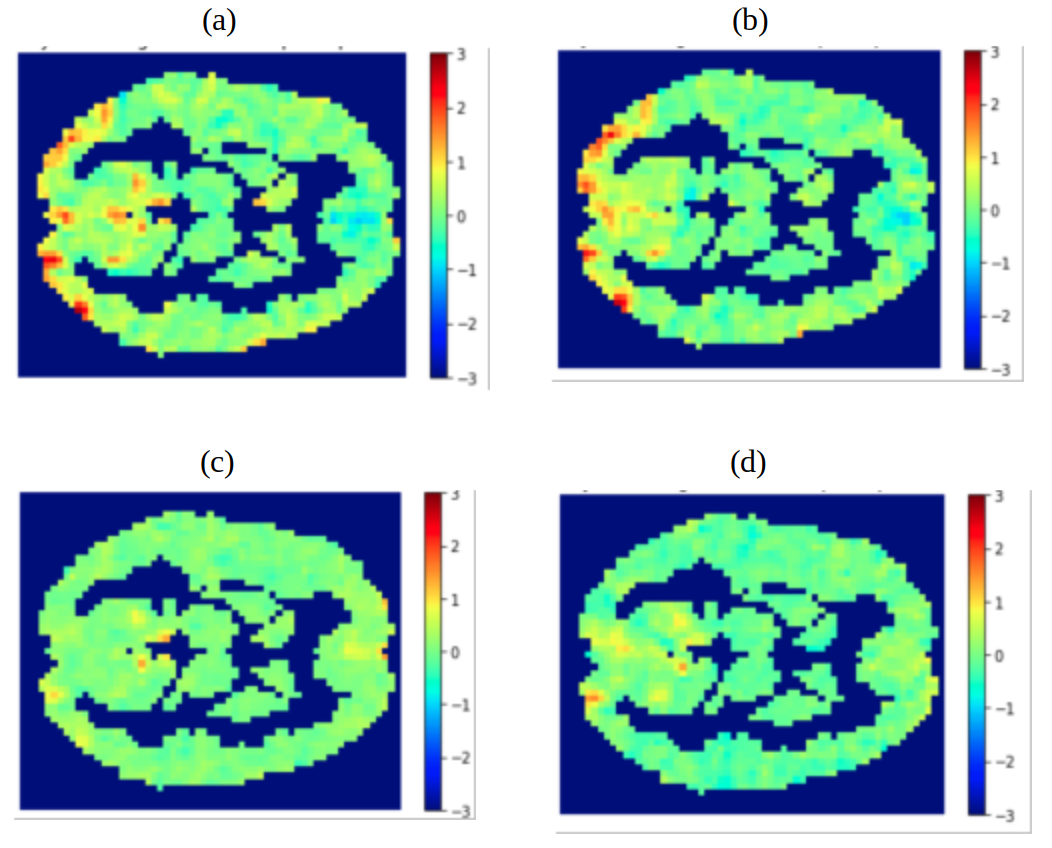
\includegraphics[scale=0.4]{brain.png}
\caption{Brain images of (a) observed 'airplane', (b) observed 'bed', (c) predicted 'airplane' (d) predicted 'bed'}
\label{brain}
\end{figure}



\paragraph{Cosine similarity score and voxel selection}
The model is evaluated by choosing the best match between the predicted and observed images of which the one with higher similarity score is considered to be a better match. The cosine similarity between two images was calculated using the top 500 voxels of the highest correlation since they are strong and repeatable in outweighing the noises. 

\section{Experiment Results}
Problematic issues exist working with fMRI data, among which the large amount of noises in the data stand out. Head movements during the capturing process is one of the largest sources leading to the noises. As can be seen in the analytic results below, the prediction accuracy varies significantly between the 9 participants. Nevertheless it's also possible that the participants have significantly different semantic interpretation of the nouns tested, we are consequently interested in using different word vector representations to verify this hypothesis in the future experiments. 

\subsection{Image prediction based on clean fMRI data set}
\paragraph{Model without regularization}
As mentioned above, the expected accuracy in matching the left-out words their observed images at chance levels should be 0.5, and an accuracy of 0.62 or higher for a single trained case is significant at $p<0.05$. We first considered the regression model without including the regularization. The accuracies of the 1770 cross-validated tests across each of the 8 participants in matching two unseen word stimuli to their fMRI images are 0.82, 0.82, 0.75, 0.74, 0.71, 0.61, 0.71 and 0.61 (mean = 0.72). Thus, \nicefrac{3}{4} participant models exhibited accuracies significantly above chance levels ($p<0.05$). On average, the model succeeded in distinguishing pairs of unseen words with accuracy around $72\%$ in the 14160 cross-validated test pairs across these nine participants. With Gaussian noises added to the insular cortex, the performance of the model becomes less preferable. The accuracies of the cross validation over all of the 8 subjects are decreased to be 0.58, 0.65, 0.69, 0.66, 0.56, 0.59, 0.56 and 0.53. Notice that the insular cortex is in fact a small region and only occupies around $1\%$ of the entire brain, the result demonstrates the sensitivity of the linear regression model and the fact that the insular cortex plays a significant role in neural representations of objects.

\paragraph{Model with regularization}
In contrast to the discussion of Mitchell, et al.\ [1], we are able to efficiently improve the performance of the model by introducing the regularization term as the Frobenius norm squared (as Figure~\ref{clean_data}). For example, with $\lambda=1.5$, the accuracies of the 1770 cross-validated tests across each of the 9 participants are improved to 0.83, 0.76, 0.76, 0.79, 0.78, 0.64, 0.75, and 0.65 (mean = 0.745). In this case, the accuracies of all of the 8 participant models are significantly above chance levels at $p<0.05$. The introduced regularization efficiently reduces the overfitting over the 8 participants, especially for the 2 participant models with worse performance previously without the regularization. The influence of $\lambda$ on the cross-validated accuracy over the 8 participants is plotted in Figure~\ref{figure1}(a). 
Furthermore, with noises included into the data, regularization can efficiently improve the performance of the linear classifier as well. As shown in Fig. ~\ref{figure1}(b), with $\lambda=1$, the optimal performance is achieved as the cross validation accuracies improved to be 0.65, 0.64, 0.65, 0.71, 0.63, 0.60, 0.66, and 0.57. Briefly, with Gaussian noises included to the insular cortex of the brain, the average accuracy across the 8 subjects is 0.64, compared to the average accuracy without regularization in the model as 0.60. 

\begin{figure}
\centering
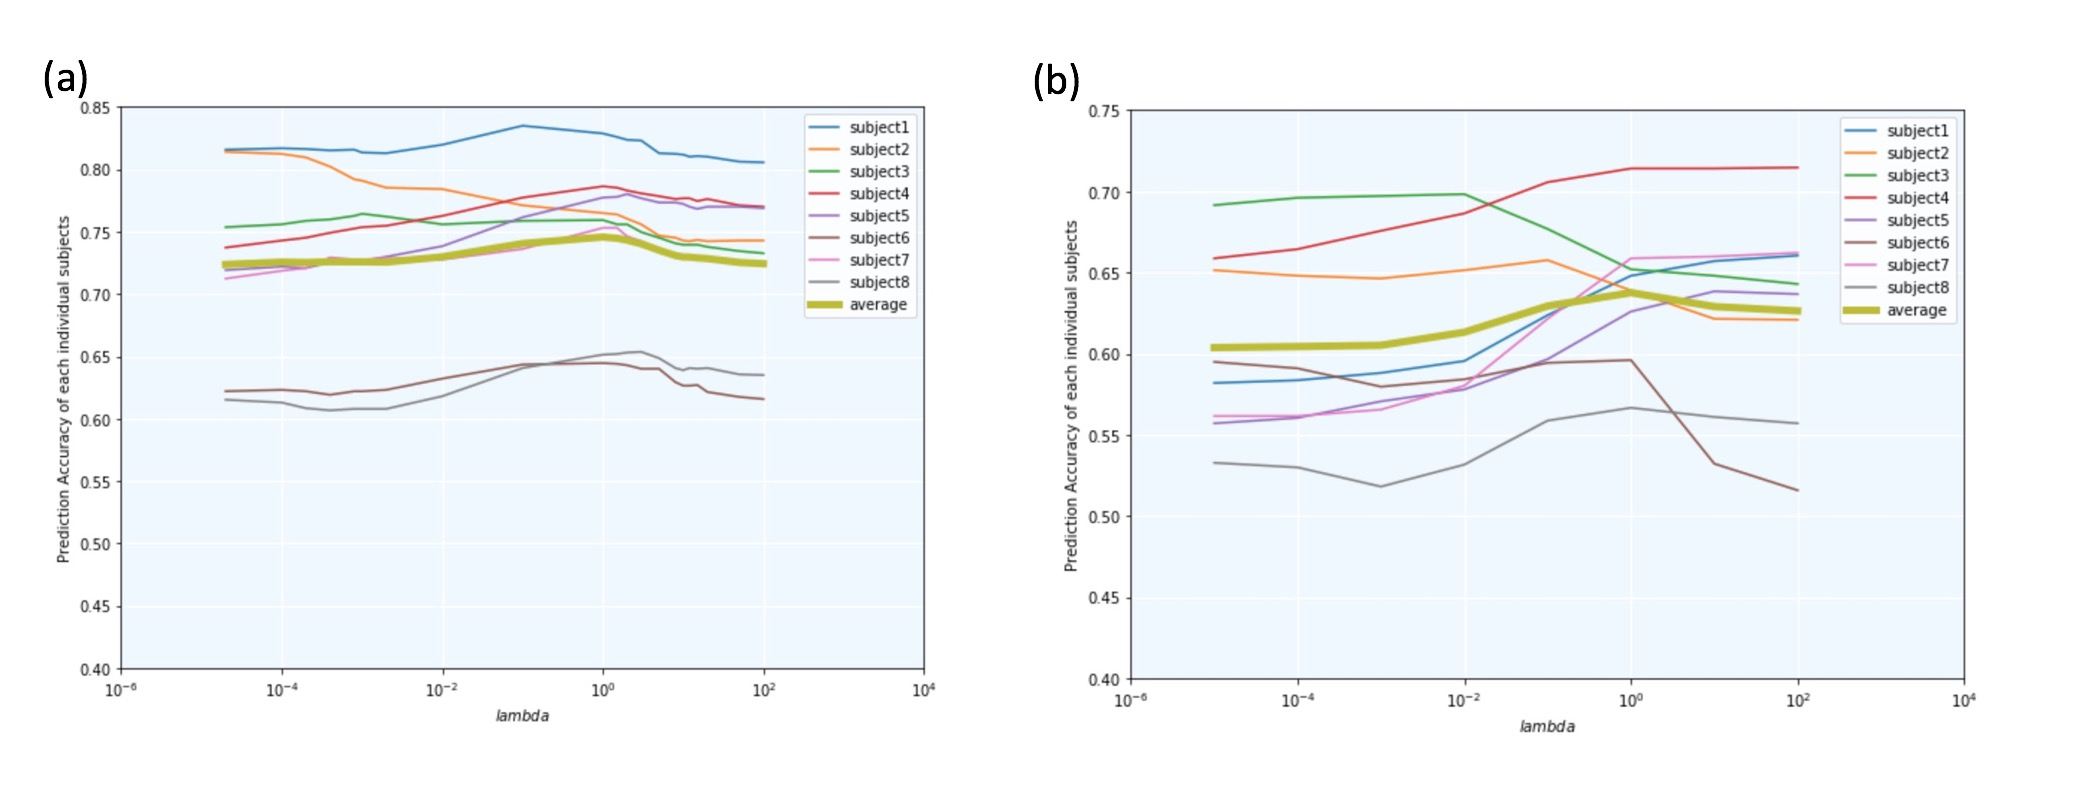
\includegraphics[scale=0.2]{figure1}
\caption{The cross-validated accuracies of 8 participants versus $\lambda$}
\label{figure1}
\end{figure}


\subsection{Image prediction based on noisy fMRI data set}
\paragraph{Noises included only into a certain class of nouns} Consider including the noises into a certain class of nouns, e.g., Gaussian noises are added only into fMRI images of the class "animal". We then proceed building the linear classifier with the noisy data as the training data set. The cosine similarity was computed for each noun using the strategy of "leave-one-out" cross validation and the average was taken within the same class afterwards. The results of the 8 subjects are shown in Fig.~\ref{noisy_data_1}(b). Albeit variation exists among the 8 subjects, especially for subject 6, we can still see a consistent pattern among the majority of the subjects. For example, nouns from the class "buildpart", "building" are least affected by the noises added in the class "animal" while "bodypart", "vegetable" and "insect" are affected strongly. This is consistent with our common sense of how the brain processes information of connected subjects.

\paragraph{Noises included only within a certain region in the brain} Consider including the noises only within the insular cortex, which is known for its function in audio-visual integration task, interoceptive awareness, hand-and-eye motor movement, swallowing, and taste perception, etc.. Notice that the insular cortex, in fact, is a small region and only occupies around $1\%$ of the entire brain. Again, we proceed building the linear classifier with the noisy data as the training data set and in this case prediction the fMRI images of each individual semantic feature as discussed above. The cosine similarity was then computed between the predicted images with and without noises included for each feature.  We take the average over 1000 iterations in this case for the predicted feature images since we found a large variation due to the randomness in the Gaussian noises included. The results of the 8 subjects are shown in Fig.~\ref{noisy_data_2}. Despite the large variation between different subjects, we see a common worse behavior of "near", "drive" and "say" among the features, which is consistent with the know brain function of insular cortex.

\begin{figure}
\centering
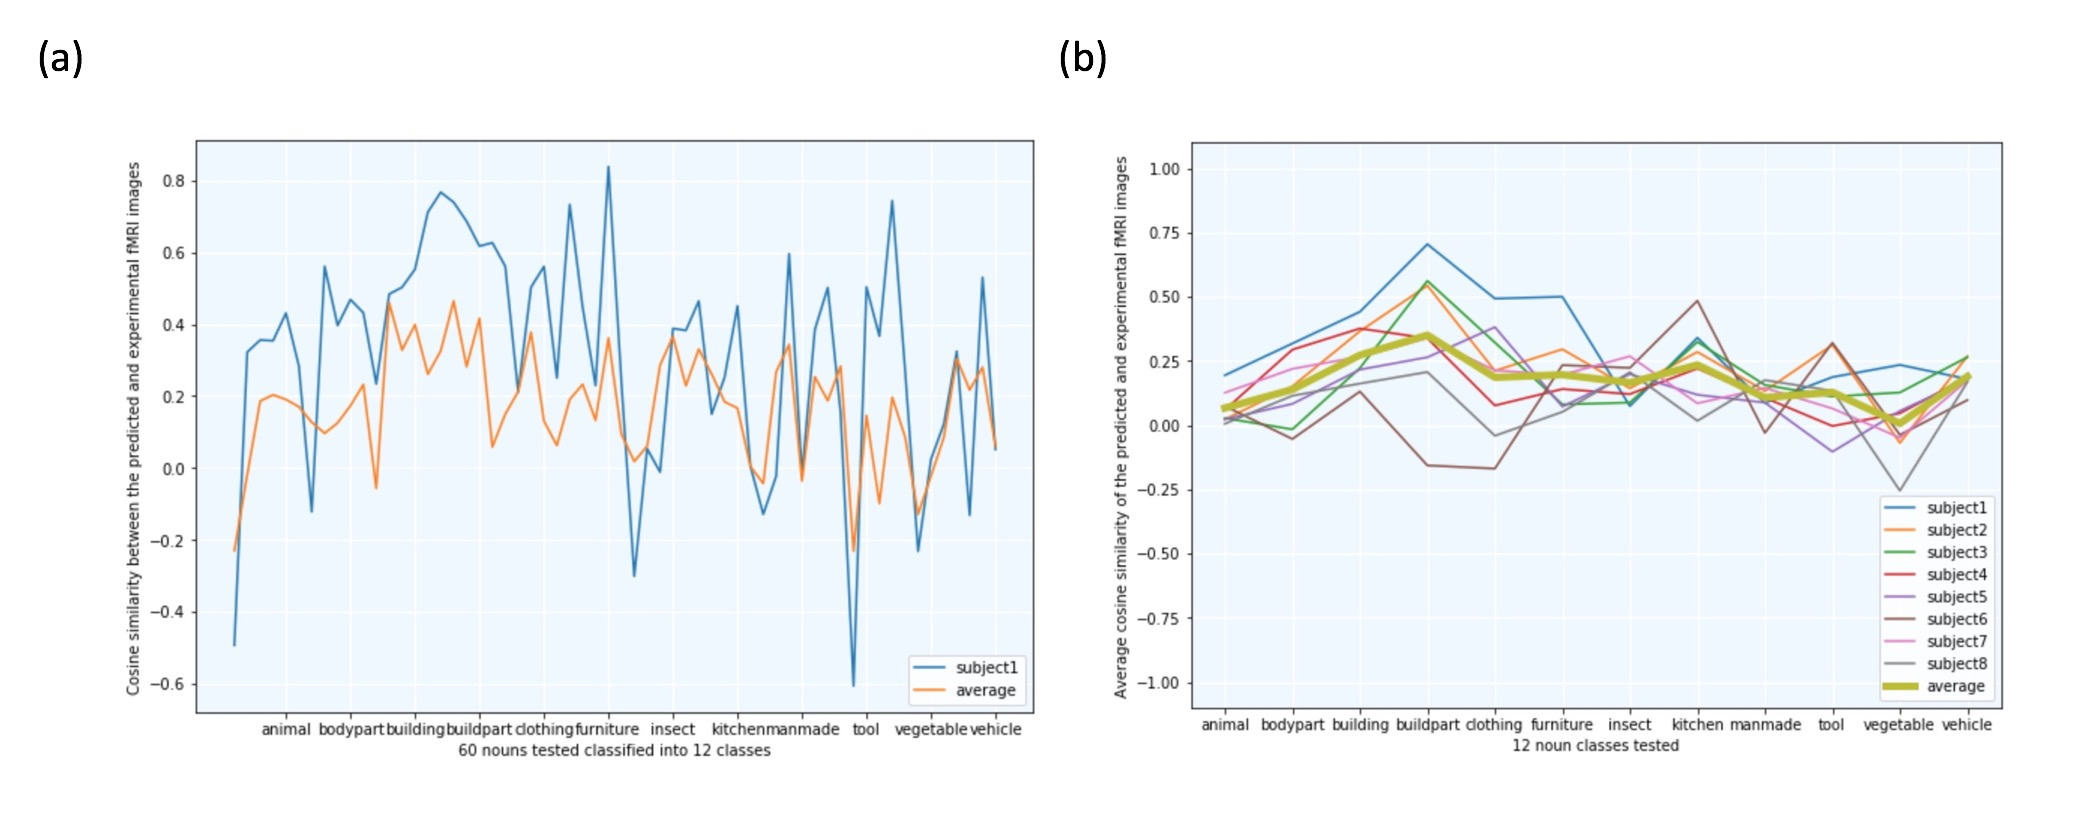
\includegraphics[scale=0.2]{noisy_data_1.jpeg}
\caption{Cosine similarity between the predicted and experimental fMRI images of 12 different classes with/out noises included. (a) Cosine similarity over 60 nouns clusters with respect to their classes of subject 1 and the average of the 8 subjects. (b) Averaged cosine similarity of the nouns within the same class of the 8 subjects.}
\label{noisy_data_1}
\end{figure}

\begin{figure}
\centering
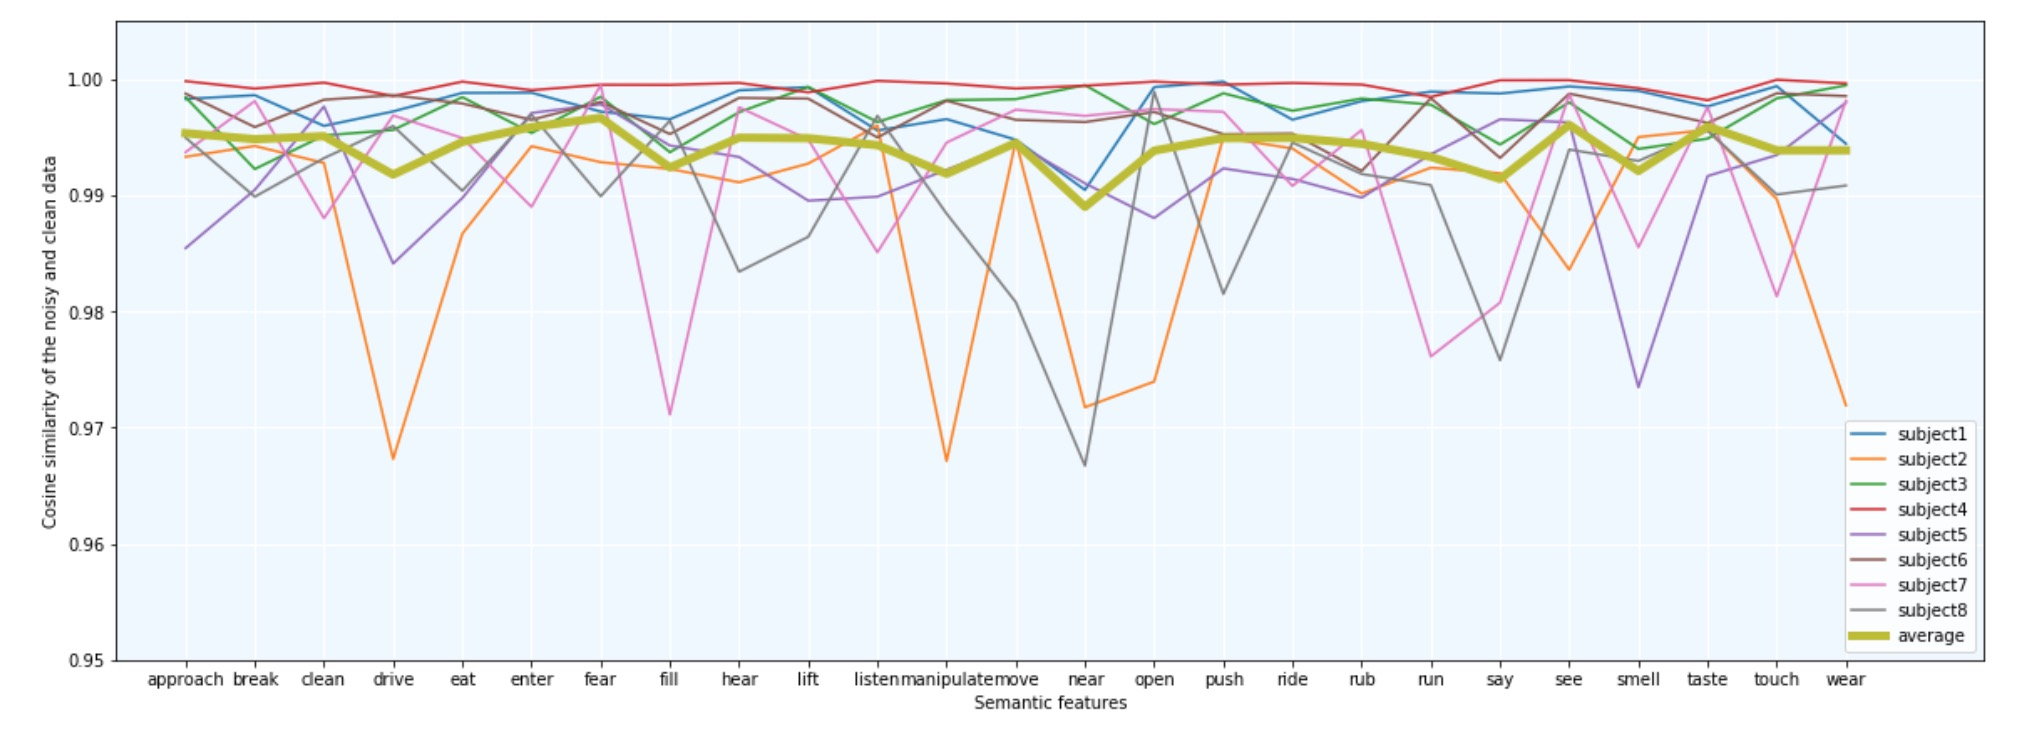
\includegraphics[scale=0.2]{noisy_data_2.jpeg}
\caption{Cosine similarity across 25 semantic features between predicted feature fMRI images with/out noises included.}
\label{noisy_data_2}
\end{figure}

\subsection{Correlation matrix}

To intuitively show the correlations between the predictions and observations, we plotted a correlation matrix for each participant and the "average participant", as Figure \ref{corr_mat} and Figure \ref{avg_corr}. Each element of the matrix is defined as the cosine similarity between the corresponding prediction and observation images. The axes in the figure are words ranked by their classes so that the words in the same class are put together.

\begin{figure}
\centering
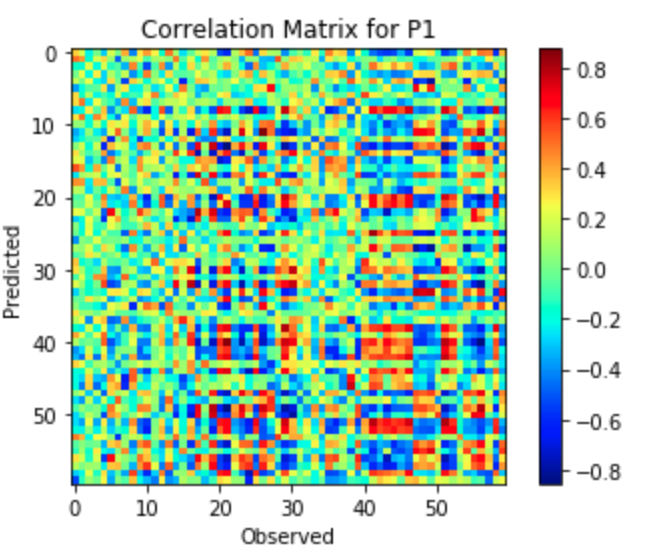
\includegraphics[scale=0.3]{P1corr.png}
\caption{The correlation matrix for P1}
\label{corr_mat}
\end{figure}

\begin{figure}
\centering
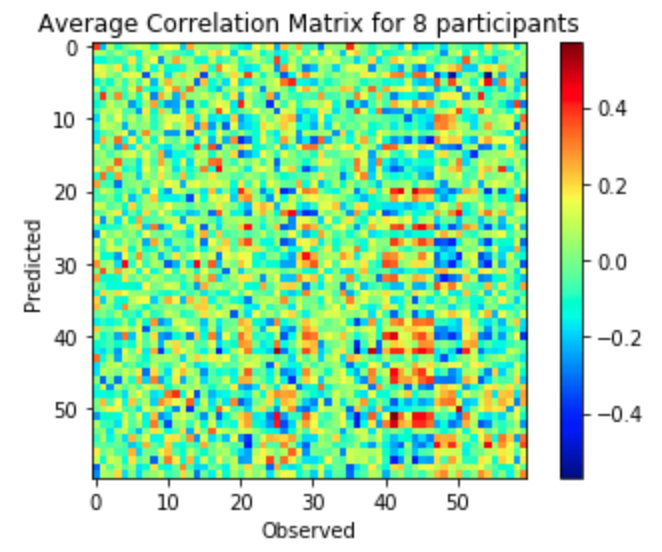
\includegraphics[scale=0.3]{avgcorr.png}
\caption{The average correlation matrix for all participants}
\label{avg_corr}
\end{figure}

We also evaluated the mean value of separately the diagonal elements and all elements of the correlation matrix for each participant and the averaged one, shown as Table \ref{table1}. From the table we can see for each participant, the mean value of the diagonal elements are much larger than that of all elements of the correlation matrix, which strongly indicates that the predicted image for a given word is more similar to the observed image for that word. 

\begin{table} 
    \centering
    \caption{{\bf Mean value for the correlation matrices}}\label{table1}
    \begin{tabular}{ccc}
    \hline
    participant & total mean & diagonal mean\\
    \hline
    P1 & 0.010 & 0.335   \\
    P2 & 0.007 & 0.258   \\
    P3 & 0.006 & 0.209   \\
    P4 & 0.005 & 0.163   \\
    P5 & 0.004 & 0.154   \\
    P6 & 0.005 & 0.110   \\
    P7 & 0.003 & 0.188   \\
    P8 & 0.002 & 0.059   \\
    average & 0.005 & 0.184   \\
    \hline
    \end{tabular}
\end{table}

\section{Conclusion}
The resulting computational model is capable of predicting the full fMRI activation image for unseen words with semantic features given with high accuracy, even with Gaussian noises included as the distortion. Albeit the performance of this computational model has large variation among different subjects, common reactions still exist and validate our assumption of the associative processing procedure in brain. Specifically, with noises added in class of "animal", we see a common pattern of weak impacts on buildings but strong impacts on human beings. Impairment on insular cortex decreases the overall prediction accuracies but it tends to have stronger impacts on semantic features related closer to its function in brain such as audio-visual integration and motor control. Nevertheless, since the choice of our semantic features are motivated by the sensory-motor features in neural representations of objects, it might explain why most of the features are affected by the change in $1\%$ voxels inside the brain. Overall, this classifier efficiently predicts the fMRI images of the unseen words, from which we can have a basic understanding of the brain function for some certain regions, as well as the association in neural representations of objects.









\section*{References}
[1] Mitchell, Tom M., et al. "Predicting human brain activity associated with the meanings of nouns." science 320.5880 (2008): 1191-1195.  

[2] Wehbe, Leila, et al. "Simultaneously uncovering the patterns of brain regions involved in different story reading subprocesses." PloS one 9.11 (2014): e112575.

[3] B. Cerf, D. LeBihan, P. F. Van de Moortele, P. Mac Leod,A. Faurion, Ann. N.Y. Acad. Sci. 855, 575 (1998).

\end{document}